% -*- coding: utf-8 -*-

\section{Rectangular Swept Spheres}
\label{rss}

\subsection{Introduction}
In this section I will go into greater detail about the RSS, how it is defined and represented, as well as the literature that I have used in this report. I will also shortly describe Oriented Bounding Boxes (OBB), Point Swept Spheres (PSS), and Line Swept Spheres (LSS), the last 2 of which are similar to RSS'. No other bounding volumes will be described. 

\subsection{Rectangular Swept Sphere}
The Rectangular Swept Sphere (RSS) is a 3D figure. It is generated by taking a sphere with a positive radius and sweeping its center over a rectangle in 3 dimensional space. This makes it resemble a rectangular rounded pillow. An illustration of a RSS can be found in figure \ref{rss-example-figure} on page \pageref{rss-example-figure}. 

\subsection{Representation of RSS}
I have chosen to represent the RSS as a rectangle in 3D together with a radius, as described in \cite{larsen00fast}, \cite{Larsen99fastproximity} and \cite{237244}. The rectangle is represented by 2 vectors, a center point. See section \ref{rectangle3d} page \pageref{rectangle3d} for  implementation details. I felt this was best way to represent it, as it adequately described the RSS, took up a minimum of space, contains the vectors, and follows the representation found in \cite{237244}, which enables me to use the axis-separation test described in \cite{237244}.

\begin{figure}
\centering
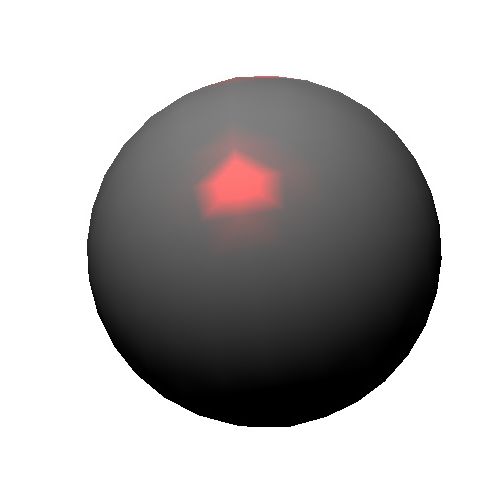
\includegraphics[width=0.5\textwidth]{figures/pss}
\caption{\label{pss-example}An example of a PSS}
\end{figure}

\subsection{Point Swept Spheres}
A point swept sphere is a BV that is created by taking a point p in 3D, and placing the center point of a sphere s with a positive radius at p. The advantage of the PSS is that it is both simple to implement and to check to for intersection with other PSS. However, PSS' can easily get a bad fit, as the properties that can be adjusted are its radius and the location of its center point. It is therefore not unthinkable that a BVH using PSS' would have a reason to perform more intersection checks than other BVs, for instance the ones mentioned in this report.

\begin{figure}
\centering
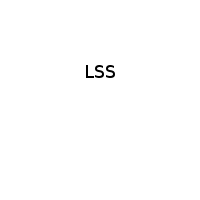
\includegraphics[width=0.5\textwidth]{figures/lss}
\caption{\label{lss-example}An example of a LSS}
\end{figure}

\subsection{Line Swept Spheres}
A line swept sphere is a BV that is created by taking a line segment l, placing the center point of a sphere s with a positive radius on one of the endpoints of l, and then sliding s to the other endpoint of l. It is a bit harder to check for intersection in LSS' than PSS' (see above), but in practice LSS' have a better fit for the points it contains, and will therefore create fewer unneeded checks for intersection than the PSS' BV.

\begin{figure}
\centering
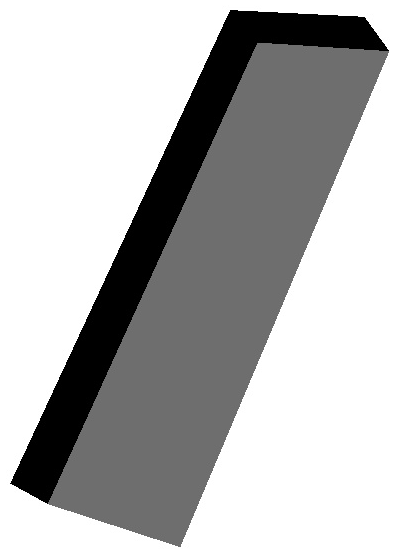
\includegraphics[width=0.5\textwidth]{figures/obb}
\caption{\label{obb-example}An example of a OBB}
\end{figure}

\subsection{OBB}
The Oriented Bounding Box is a Box of a certain positive height, width and length, and which has an orientation - i.e. is not necessarily axis-oriented. For an example of an OBB, see figure \ref{obb-example}. As I will explain later, RSS' and OBB's based on the same point set should have a similar volume - with the RSS in most cases having a volume that is slightly larger. 

\subsection{Literature used in this report}
\label{lit}
For this project I have used the following literature:
\begin{description}
\item[\cite{larsen00fast}] Gives an introduction on how to perform a fast distance query between RSS' with a pruning method that eliminates at least half of the tests. The article only gives a brief overview of the pruning method, the reasoning behind it and how to perform it in practice, and refers to \cite{Larsen99fastproximity} (by the same authors) for more detail. There is also a brief description of an alternative method to the Axis-separation used in this project, to detect whether 2 RSS' overlap, employed the property of slabs. The slab-method seems like it could be far more effective than the Axis-separation test, but I have not attempted to implement it, as I have overlooked it (it is not described in any great detail, and comes after a reference to \cite{Larsen99fastproximity}, making it seem like an afterthought).   

\item[\cite{Lotan03algorithmand}] Gives a general introduction to Monte Carlo simulation of Proteins, as well as a comparison of several BV's and the algorithms for these, for protein folding. Nothing in this article is used directly, but rather as background material for the domain.

\item[\cite{Larsen99fastproximity}] Gives an more in-depth exploration of the minimum distance calculations mentioned \cite{larsen00fast}, as well as an overview of the method they have used to generate the RSS' using OBBs. While the explanation of the pruning method is mostly explained to be both convincing and implementable, there is 1 case (out of 3) where the article explicitly mentions that ``needs extra analysis for closest point test'' (\cite{Larsen99fastproximity} section 4.3.1, page 14), but is not further elaborated upon. \cite{Larsen99fastproximity} also tries to explain the slab-method mentioned in \cite{larsen00fast} in greater detail, but the way the explanation is structured makes it possible for the reader to think that they were using the Axis-separation method to find out whether the 2 RSS' are separated or not. The description of the slab-method itself is also not very specific, and does not explicitly mention the radius property of the RSS (instead preferring to focus in which cases the 2 rectangles of the RSS' are overlapping).

\item[\cite{237244}] Gives a description of the axis-separation test for OBB's, as well as a description on how to optimize the checks.
\end{description}

\subsection{Conclusion}
I have in this section described the Rectangular Swept Sphere, as well as the 3 other BV that I that I will work with throughout this report. I have furthermore given an example of all 4 BVs, and shortly discussed the main literature, that I have used for this project.
